\documentclass{article}
\usepackage{../settings}

\begin{document}
\hexcover{兩天一夜中南部行}{暑假作業}{作者:曾嘉禾}{Violet}{國文}

\begin{large}
\begin{boxpar}{Violet}{第一站:彰化王功食海鮮}
在從新竹出發後的剛開始,經過了彰化的王功。據說在那裡有神秘的宮廟文化,以及因為靠近海邊的關係而盛產海鮮。其中,店外大大的橫幅「蚵仔披薩」吸引了我的目光。所以我們一家人就去那家餐廳消費。雖然最後沒有點蚵仔披薩,但是店內的其他項目也十分誘人。例如鮮甜的絲瓜香菇,香氣十足的蛤蜊清湯,又大又肥的鮮蝦等。經過美一道菜的味蕾轟炸後感到極為滿足。
\begin{imgbox}{吃飯.jpg}
    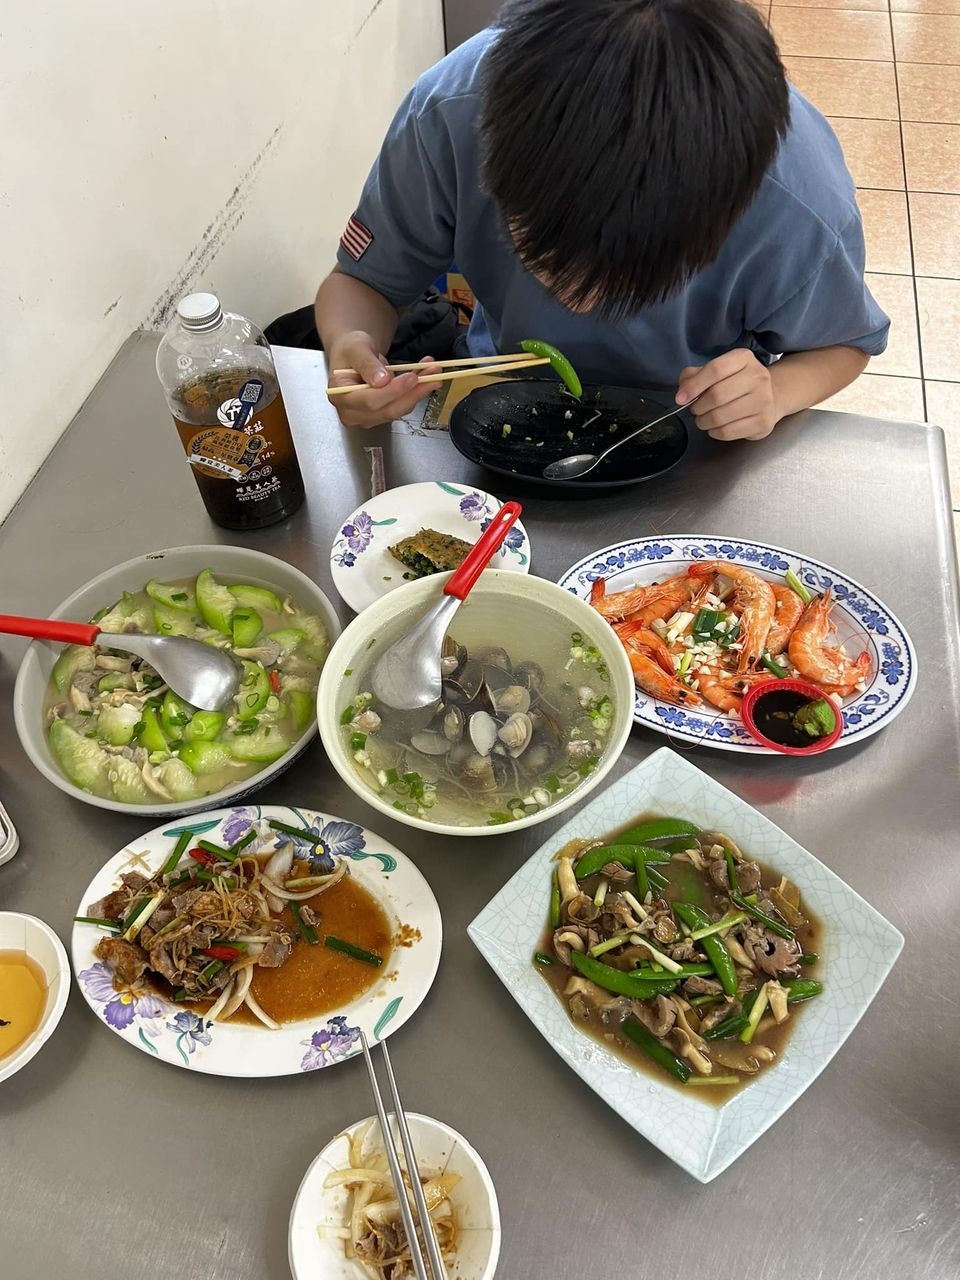
\includegraphics[width=0.65\textheight]{src/seafood.jpg}
\end{imgbox}

\end{boxpar}
    \begin{boxpar}{Violet}{第二站:嘉義旺來山}
        國中一年級時,去了嘉義旺來山的許願區許願自己考上好高中。到了三年後,我的確考上了第一志願:師大附中。雖然當時承諾會去還願,但因為時間的限制而無法這麼做。直到在這次暑假才有機會回訪旺來山。在這次旅程不但不食言地在旺來山還願,還許下新的願望:考上心中的理想台大電機系。
    \end{boxpar}
    \begin{boxpar}{Violet}{第三站:台中雪山—稍來山}
        稍來山是一座小百岳。當時去的時候繞了好一陣子的山路才到那邊。神奇的是,據說雪山國家公園為了讓垃圾不留山中而少有餐廳。換句話說遊客必須自己準備午餐,不然會在山上餓肚子。這件事情讓我大開眼界。
    \end{boxpar}

\end{large}
\end{document}
